\subsection{Methods}\label{sec:m4:methods}
    First things first, we are going to calculate a lot of spherical Bessel functions, since we need to integrate these across $x$ in finding the transfers function (for every $k$). Thus, it is computationally wise to spline them in advance. Further, we need to calculate the line of sight integral across all the $x$-values in order to obtain the transfer function. We may choose to compute the transfer function direction when integrating the power spectrum, or we may precompute it and then spline the result. We will choose the latter. Lastly, we integrate and compute $C_l$ as functions of $l$. We expect this to be relatively smooth function, so we choose a small finite number of $l$-s for which we perform the integral. 
    The $l$-s we are going to use are the following:

    $l\in$ [2,    3,    4,    5,    6,    7,    8,    10,   12,   15,   
    20,   25,   30,   40,   50,   60,   70,   80,   90,   100,  
    120,  140,  160,  180,  200,  225,  250,  275,  300 \dots 2000],
    where the dots represent increments of 50. 
    \subsubsection{Making Bessel splines}
        We may precompute and spline the spherical Bessel function since we know the minimal and maximum value of its argument. This is, we need to compute for values of $z\equiv k(\eta_0-\eta(x))$ where $\eta_0$ is the current value. From ~\cref{fig:m1:cosmic_conformal_time} we have that $\eta(x) \leq \eta_0$ for $x\leq0$,\footnote{The line of sight integration is from early times until today, so we do not need to think about future value, hence $x\leq0$.} so it becomes apparent that we need to precompute values for $z\in[0, \eta_0k_\mathrm{max}]$ for every $l$. Since the spherical Bessel functions oscillate with a period of approximately $2\pi$, we need to take enough samples in order to account for all effects. If we want $n$ samples per oscillation we need to sample with a rate:
        \begin{equation}\label{eq:m4:methods:bessel_sampling}
            \Delta z = \frac{2\pi}{n_\mathrm{bessel}}.
        \end{equation}
        We will use $n_\mathrm{bessel}=25$ and the result may be seen in ~\cref{fig:m4:bessel}, from which we clearly see that we sample with enough accuracy. The first peaks occur at around the value of the order of the function. 
        \begin{figure}
            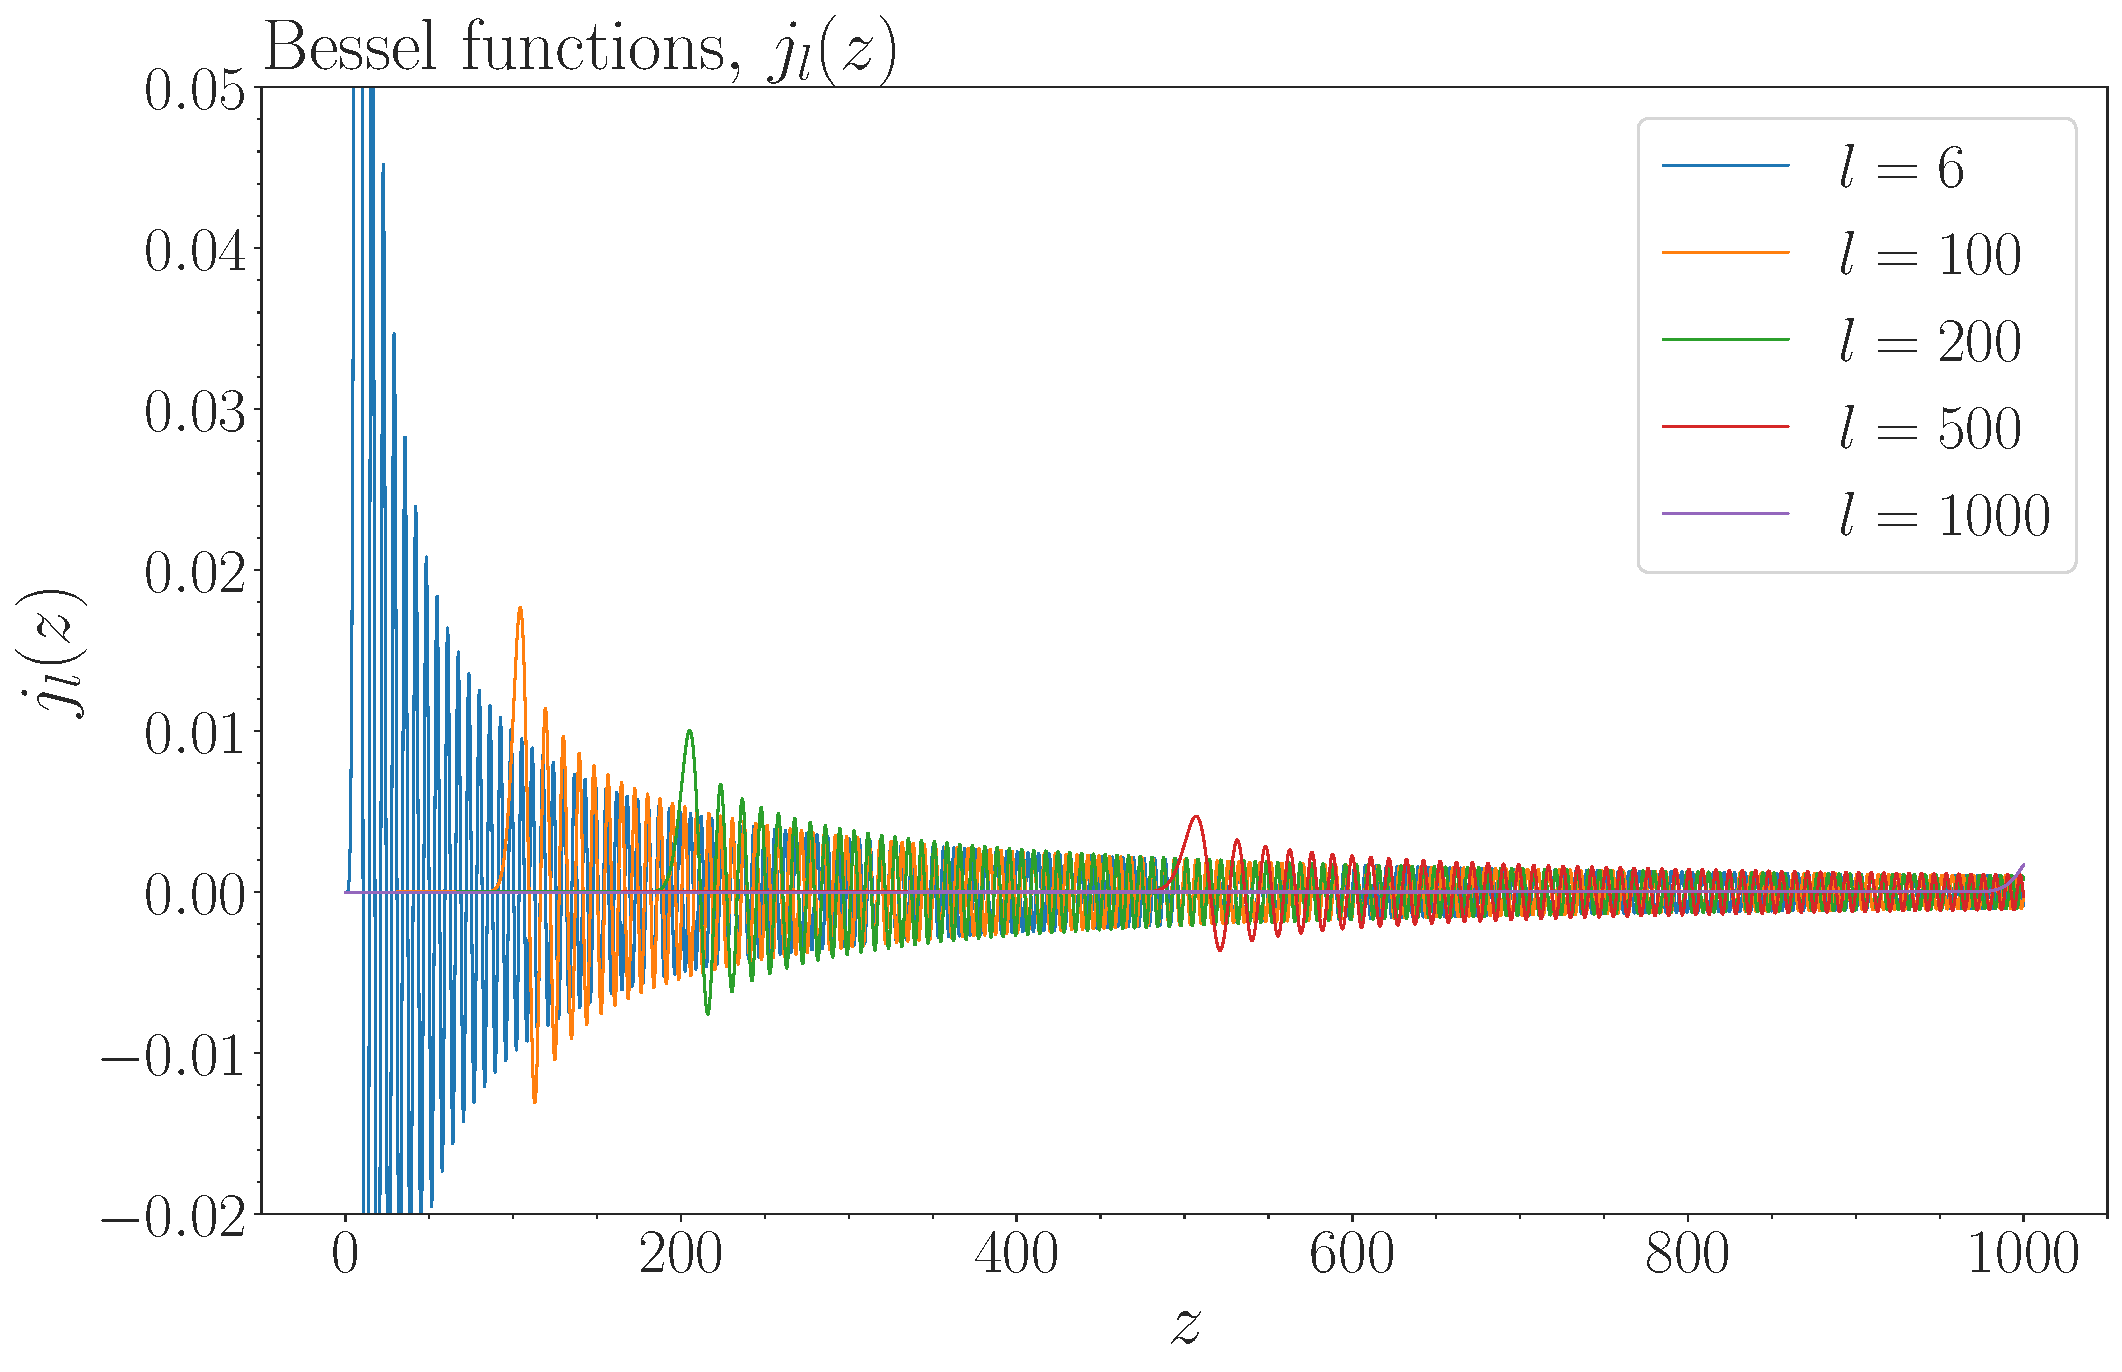
\includegraphics[width=\linewidth]{bessel.pdf}
            \caption{The spherical Bessel function for selected $l$-values.}
            \label{fig:m4:bessel}
        \end{figure}
        One ending note is that if the argument $z$ of the spherical Bessel functions are too large, some functions for finding it may break down, so proceed with caution. 

    \subsubsection{Line of sight integration}
        We are now ready to perform the actual line of sight integration from ~\cref{eq:m3:theory:line_of_sight_integral_definition}. We are supposed to integrate from $-\infty$ until today, but by investigating the integrand we may simplify this. ~\cref{fig:m4:LOS_integrand} show the integrand for a selected number of $l$-s. From the discussion of the source function in ~\cref{sec:m3:theory:line_of_sight}, we would expect most of its contribution to be around the time of recombination. This is emphasized in the plot, and we also see some effects at later times, up until today. These are the correction effects to the source function, which we need to take into account. The take home message is that there is very limited contribution from the time before recombination, so we choose some time right before recombination from which we start the integration. We must also here pay close attention to the sampling of the integrand because of the oscillations, and because it is a function of both $x$ and $k$. We sample w.r.t. $x$ as follows:
        \begin{equation}
            \Delta x = \frac{2\pi}{n_\mathrm{LOS}^{(x)}},
        \end{equation}
        and w.r.t. $k$ as:
        \begin{equation}
            \eta_0\Delta k = \frac{2\pi}{n_\mathrm{LOS}^{(k)}},
        \end{equation}
        where we use $n_\mathrm{LOS}^{(x)}=350$, and $n_\mathrm{LOS}^{(k)}=32$, since the integrand is a lot smoother in $k$ than $x$, we thus need a rather high resolution in $x$. 

        \begin{figure}
            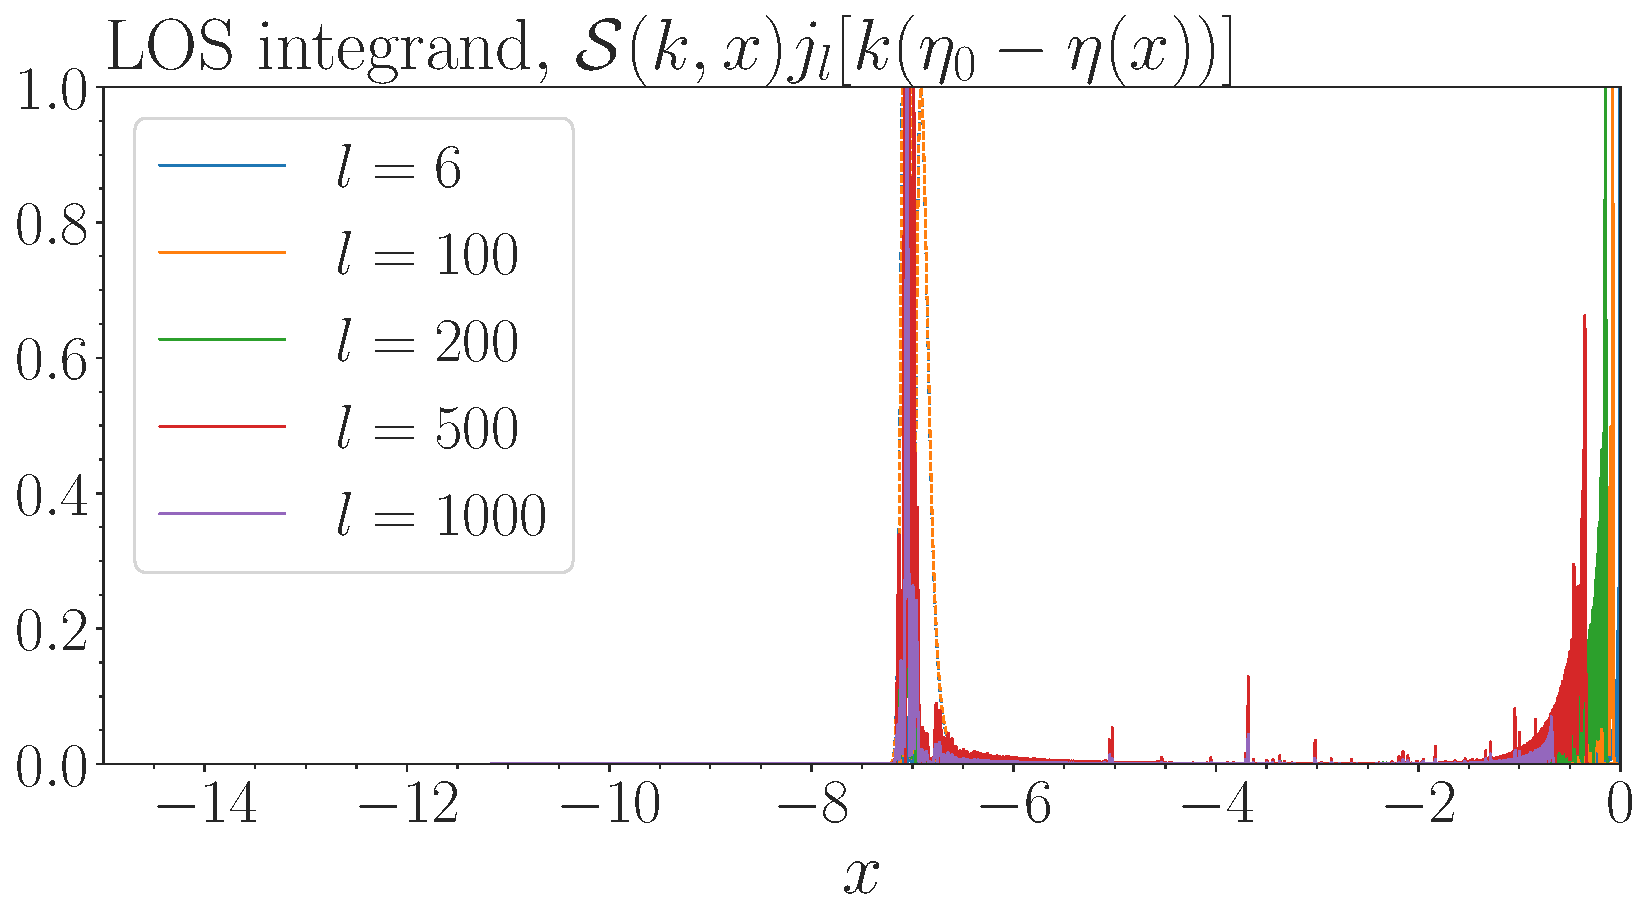
\includegraphics[width=\linewidth]{LOS_integrand.pdf}
            \caption{Integrand of LOS integral, mostly governed by the source function. The contribution is very limited before, but peaked during recombination. We have some contribution between recombination and today due to the corrections to the source function. The plot shows (but indistinguishable) values for $k=k_\mathrm{min}$ and $k=k_\mathrm{max}$ in order to highlight the extreme effects.}
            \label{fig:m4:LOS_integrand}
        \end{figure}

        The result of the line of sight integral is the transfer function $\T_l(k, \eta=\eta_0)$, and can be seen for the same selected values of $l$ in ~\cref{fig:m4:transfer_function}. It appears that our sampling was successful as we have captured the oscillations. This is by far the most time-consuming part of the integration, and the result is thus splined for easy access later on. 
        \begin{figure}
            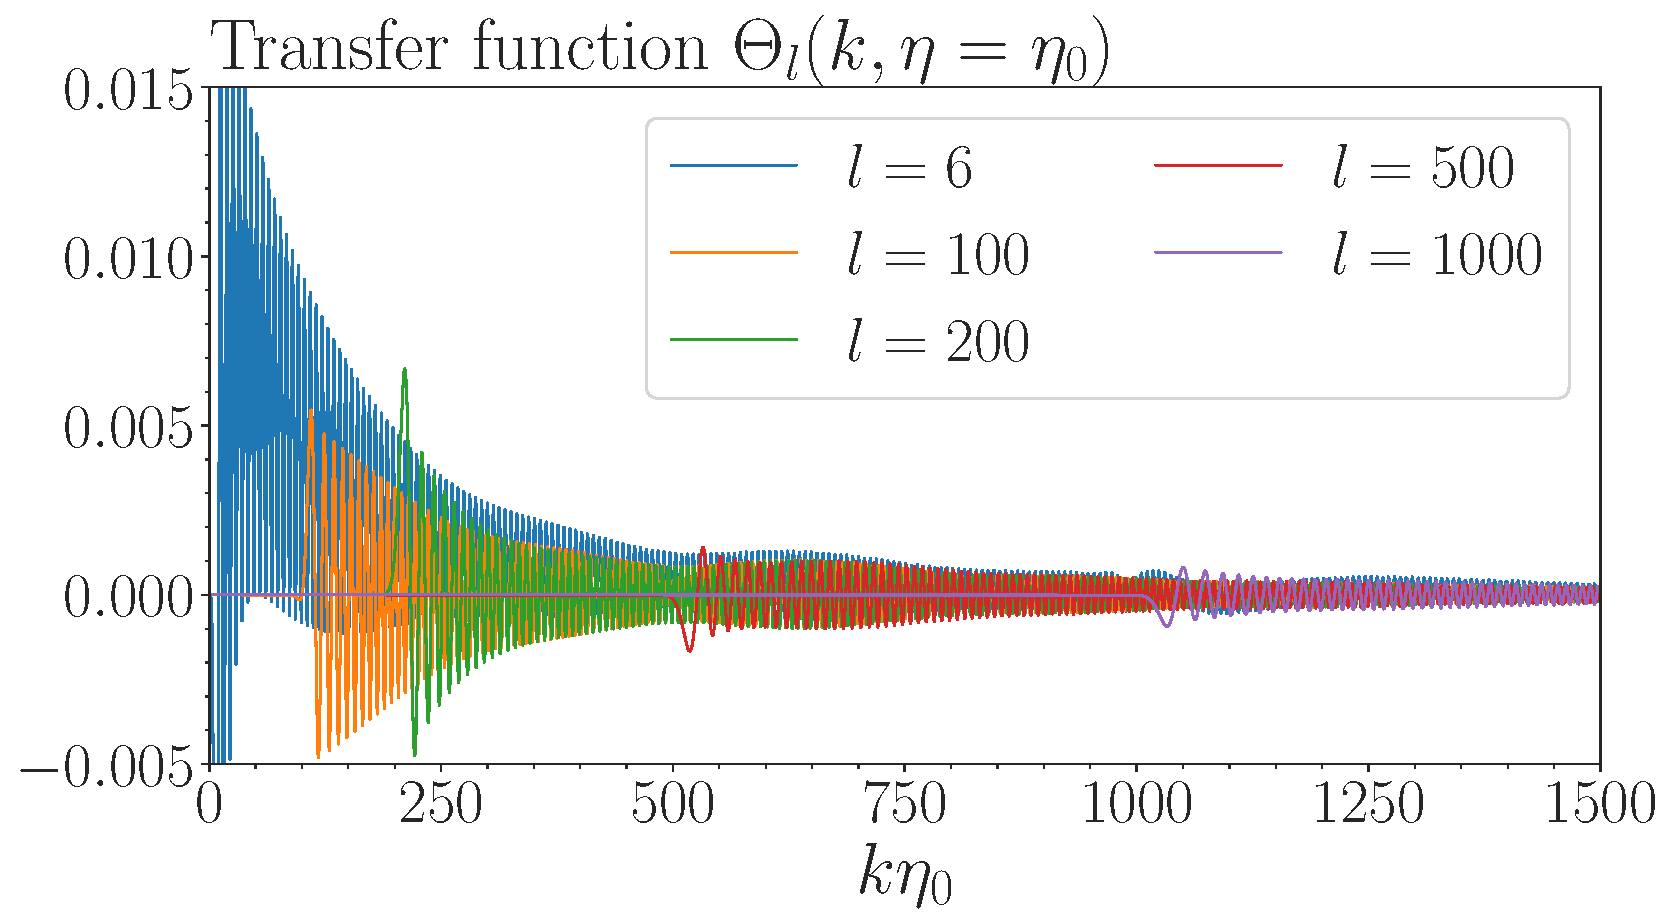
\includegraphics[width=\linewidth]{transfer_function.pdf}
            \caption{Transfer function after performing line of sight integration for a selected number of $l$-s, as function of $k$. }
            \label{fig:m4:transfer_function}
        \end{figure}
    \subsubsection{Integrate across $k$}
        When integating across $k$ in order to obtain the power spectrum $C_l$ the main dependence on $k$ is through the transfer function, so we use the same resolution as earlier for $k$. It is worth noting that integrating with respect to $\d k/k$ is equivalent to integrating with respect to $\d(\log{k})$, as long as we use the correct limits. It is thus straightforward to compute the angular power spectrum in ~\cref{eq:m4:theory:power_spectrum_logk}, and it is not very time-consuming since we have precomputed the transfer function already. ~\cref{fig:m4:C_l_integrand} shows the integrand of the angular power spectrum integral, which is just the transfer function weighted by $k$ (the primordial power spectrum is not included). 
        \begin{figure}
            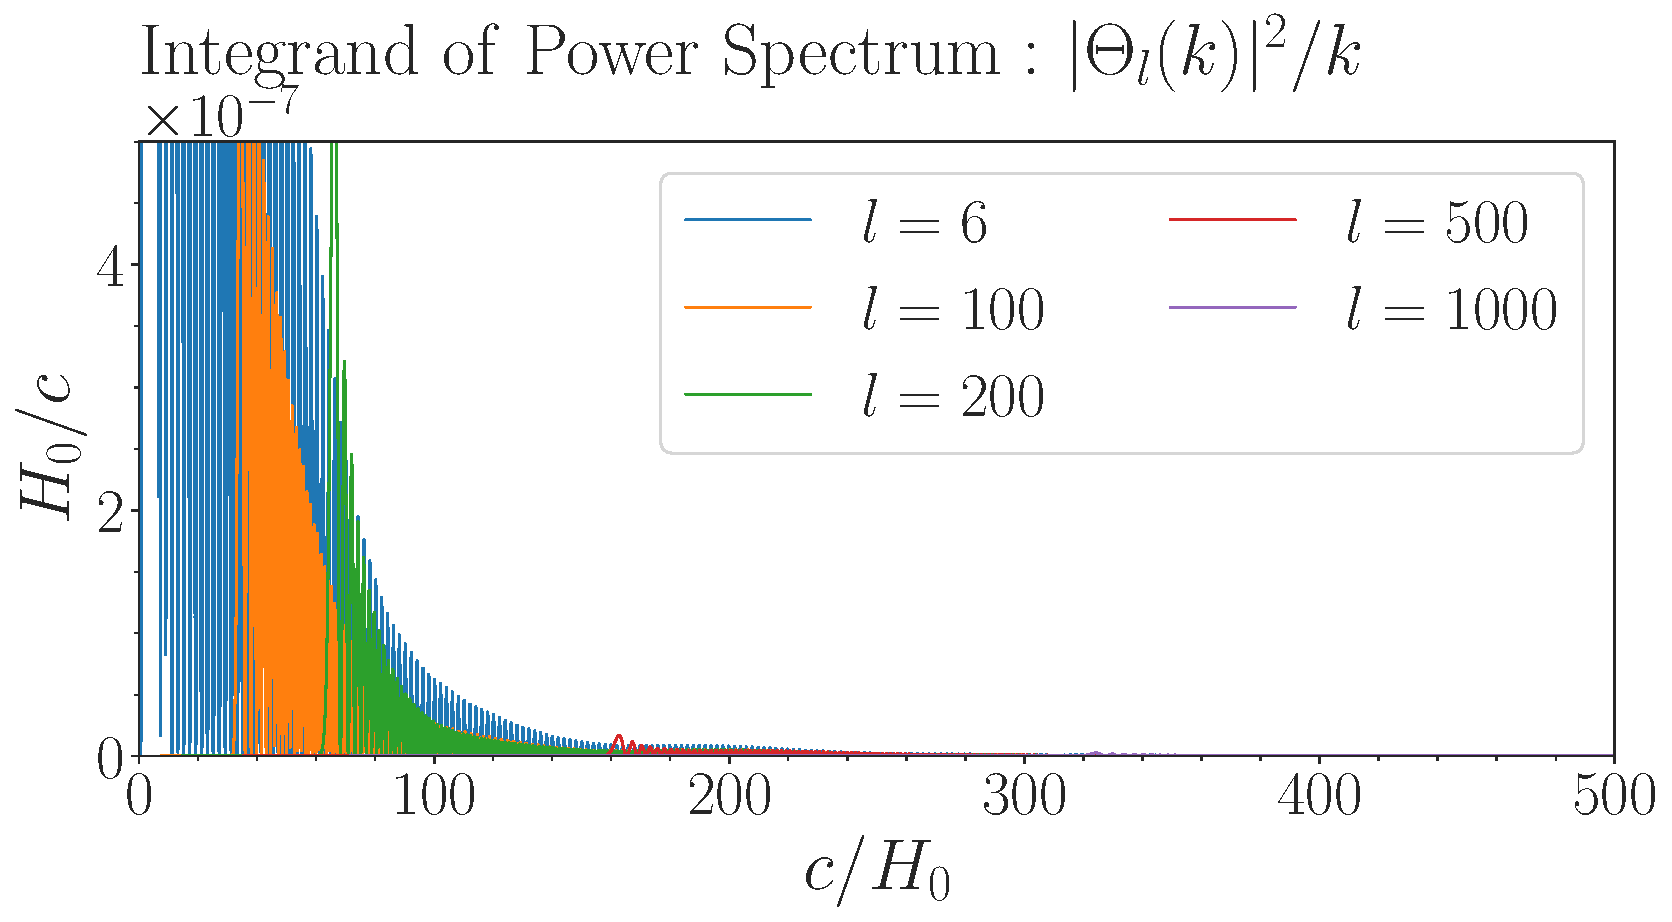
\includegraphics[width=\linewidth]{C_l_integrand.pdf}
            \caption{Integrand of the power spectrum integral as function of $k$, given for a selected number of $l$-s.}
            \label{fig:m4:C_l_integrand}
        \end{figure}


    \subsubsection{Numerical integration}
        Due to the large sampling rate when the functions are not smooth, there is no point in wasting computational resources on a more accurate numerical integrator than the \textit{trapezoidal method}. Since we specify samplings as constant spacing, we end up with a uniformly spaced domain, where we have $N$ discretised spaces and $N\Delta x= b-a$ where $b$ is the maximum value of the domain and $a$ the minimum. We approximate the finite integral as follows:
        \begin{equation}
            \int_a^bf(x)\d x \approx \left[ \sum_{i=1}^{N-1}f(x_i) + \frac{f(x_a)+f(x_b)}{2} \right]\Delta x.
        \end{equation}
        This method is used both when integrating across $x$ and $k$. 


